\chapter{Ecuaciones diferenciales de primer orden}

Una \textbf{ecuación diferencial} relaciona una función desconocida con sus derivadas. Son el lenguaje natural de las leyes que describen cómo cambia una cantidad: la razón a la que crece una población, la temperatura de un cuerpo que se enfría, la corriente en un circuito. Resolver una de ellas es, en el fondo, el problema inverso de derivar —una integración generalizada—, de modo que este capítulo se apoya directamente en las técnicas de integración (Capítulo~\ref{cap:tecintegracion} y siguientes) y en el modelado con razones de cambio del cálculo diferencial.

Este es el primero de cinco capítulos dedicados a las ecuaciones diferenciales: las de \textbf{primer orden} (este capítulo), las \textbf{lineales de orden superior}, los \textbf{sistemas} de ecuaciones, las soluciones por \textbf{series de potencias} y la \textbf{transformada de Laplace}. Empezamos por el primer orden, donde una sola integración —cuando es posible— basta para hallar la solución, y donde ya aparecen las dos ideas que vertebran todo el bloque: el \emph{teorema de existencia y unicidad} y la interpretación \emph{cualitativa} mediante el campo de pendientes.

\section{Definiciones básicas}

\begin{definition}
Una \textbf{ecuación diferencial ordinaria (EDO)} es una ecuación que involucra una función desconocida \(y(x)\) y algunas de sus derivadas. El \textbf{orden} de la EDO es el orden de la derivada más alta que aparece. El \textbf{grado} es el exponente al que está elevada la derivada de mayor orden, siempre que la ecuación sea polinómica en las derivadas.
\end{definition}

\begin{definition}
Una EDO es \textbf{lineal} si puede escribirse como
\[
a_n(x)y^{(n)} + a_{n-1}(x)y^{(n-1)} + \cdots + a_1(x)y' + a_0(x)y = g(x),
\]
donde \(a_i(x)\) y \(g(x)\) son funciones de \(x\) únicamente. Si no es de esta forma, se dice \textbf{no lineal}.
\end{definition}

\begin{definition}
Una \textbf{solución general} de una EDO de orden \(n\) es una familia de soluciones que depende de \(n\) constantes arbitrarias. Una \textbf{solución particular} se obtiene asignando valores específicos a dichas constantes, a menudo mediante condiciones iniciales.
\end{definition}

\begin{definition}
Un \textbf{problema de valor inicial (PVI)} consiste en una EDO junto con condiciones que especifican el valor de la función y sus derivadas hasta el orden \(n-1\) en un punto dado \(x_0\):
\[
y(x_0)=y_0,\quad y'(x_0)=y_1,\quad \dots,\quad y^{(n-1)}(x_0)=y_{n-1}.
\]
\end{definition}

Antes de resolver una EDO conviene \emph{verla}. Una EDO de primer orden \(y'=f(x,y)\) asigna a cada punto \((x,y)\) del plano una pendiente \(f(x,y)\); el conjunto de esos pequeños segmentos es el \textbf{campo de pendientes}, y toda curva solución debe ser tangente al campo en cada uno de sus puntos. La Figura~\ref{fig:campo_pendientes} muestra el campo de \(y'=x-y\) con tres soluciones superpuestas: aun sin resolver la ecuación, el dibujo revela que todas las soluciones se aproximan a la recta \(y=x-1\).

\begin{figure}[H]
\centering
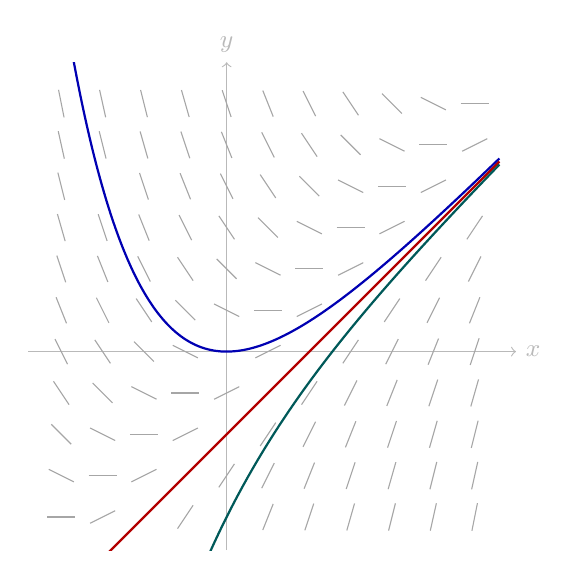
\begin{tikzpicture}[scale=1.05]
\draw[->,gray!55] (-2.4,0)--(3.5,0) node[right]{\small $x$};
\draw[->,gray!55] (0,-2.4)--(0,3.5) node[above]{\small $y$};
\foreach \x in {-2,-1.5,...,3}{
  \foreach \y in {-2,-1.5,...,3}{
    \pgfmathsetmacro{\m}{\x-\y}
    \pgfmathsetmacro{\ang}{atan(\m)}
    \draw[gray!70] ({\x-0.17*cos(\ang)},{\y-0.17*sin(\ang)})--({\x+0.17*cos(\ang)},{\y+0.17*sin(\ang)});
  }
}
\begin{scope}
\clip (-2.4,-2.4) rectangle (3.5,3.5);
\draw[blue!70!black,thick,smooth,samples=100,domain=-2:3.3] plot(\x,{\x-1+exp(-\x)});
\draw[red!70!black,thick,smooth,samples=100,domain=-2:3.3] plot(\x,{\x-1});
\draw[teal!70!black,thick,smooth,samples=100,domain=-2:3.3] plot(\x,{\x-1-exp(-\x)});
\end{scope}
\end{tikzpicture}
\caption{Campo de pendientes de \(y'=x-y\) con tres curvas solución \(y=x-1+Ce^{-x}\) (\(C=1,0,-1\)). Todas convergen a la recta \(y=x-1\) (\(C=0\), en rojo) cuando \(x\to\infty\).}
\label{fig:campo_pendientes}
\end{figure}

El campo de pendientes sugiere que por cada punto pasa exactamente una curva solución. Esto no es casual: es el contenido del teorema fundamental del capítulo.

\begin{theorem}[Existencia y unicidad (Picard--Lindelöf)]\label{thm:cap27:existencia-unicidad}
Sean \(f(x,y)\) y \(\partial f/\partial y\) continuas en un rectángulo
\[
\mathcal{R}=\{(x,y):|x-x_0|\le a,\ |y-y_0|\le b\}.
\]
Entonces el problema de valor inicial
\[
y'=f(x,y),\qquad y(x_0)=y_0,
\]
posee una \emph{única} solución \(y=\varphi(x)\) definida en algún intervalo \(|x-x_0|\le h\) con \(h\le a\).
\end{theorem}

\begin{rem}
La demostración se apoya en la \textbf{iteración de Picard}: se reescribe el PVI como la ecuación integral
\[
y(x)=y_0+\int_{x_0}^{x} f\bigl(t,y(t)\bigr)\,dt
\]
y se construye la sucesión \(\varphi_0(x)=y_0\), \(\varphi_{n+1}(x)=y_0+\int_{x_0}^{x} f\bigl(t,\varphi_n(t)\bigr)\,dt\). La continuidad de \(\partial f/\partial y\) hace del operador integral una contracción, con lo que \(\varphi_n\) converge uniformemente a la única solución.

La hipótesis sobre \(\partial f/\partial y\) es esencial para la \emph{unicidad}. Por ejemplo, el PVI \(y'=y^{2/3}\), \(y(0)=0\), tiene \(\partial f/\partial y=\tfrac{2}{3}y^{-1/3}\) no acotada cerca de \(y=0\) y admite \emph{dos} soluciones: \(y\equiv 0\) y \(y=\bigl(\tfrac{x}{3}\bigr)^{3}\).
\end{rem}

\section{Ecuaciones de variables separables}

Una EDO de primer orden es de \textbf{variables separables} si puede escribirse como
\[
\frac{dy}{dx} = f(x)g(y).
\]
Para resolverla, separamos las variables:
\[
\frac{dy}{g(y)} = f(x)\,dx,
\]
e integramos ambos lados:
\[
\int \frac{dy}{g(y)} = \int f(x)\,dx + C.
\]

\begin{example}[Crecimiento poblacional de Malthus]
La población \(P(t)\) de una especie en un entorno sin limitaciones de recursos satisface
\[
\frac{dP}{dt} = kP,
\]
donde \(k\) es la tasa de crecimiento constante. Resolver el PVI con \(P(0)=P_0\).

\begin{myproof}
\textbf{Paso 1.} Separar variables:
\[
\frac{dP}{P} = k\,dt.
\]

\textbf{Paso 2.} Integrar:
\[
\int \frac{dP}{P} = \int k\,dt \quad\Longrightarrow\quad \ln|P| = kt + C_1.
\]

\textbf{Paso 3.} Despejar \(P\):
\[
|P| = e^{kt+C_1} = e^{C_1}e^{kt} \quad\Longrightarrow\quad P = C e^{kt},
\]
con \(C = \pm e^{C_1}\).

\textbf{Paso 4.} Usar la condición inicial \(P(0)=P_0\):
\[
P_0 = C e^{0} = C \quad\Longrightarrow\quad P(t) = P_0 e^{kt}.
\]
Por tanto, la solución del PVI es
\[
\boxed{P(t) = P_0 e^{kt}}.
\]
\end{myproof}
\end{example}

\begin{example}[Decaimiento radiactivo]
Una sustancia radiactiva se desintegra a una tasa proporcional a la cantidad presente. Si inicialmente hay \(Q_0\) gramos y después de 10 años quedan \(0.8Q_0\), determinar la vida media.

\begin{myproof}
\textbf{Paso 1.} Modelo: \(\frac{dQ}{dt} = -kQ\), \(k>0\). Separando:
\[
\frac{dQ}{Q} = -k\,dt.
\]

\textbf{Paso 2.} Integrar:
\[
\ln|Q| = -kt + C \quad\Longrightarrow\quad Q(t) = Q_0 e^{-kt}.
\]

\textbf{Paso 3.} Usar \(Q(10)=0.8Q_0\):
\[
0.8Q_0 = Q_0 e^{-10k} \quad\Longrightarrow\quad e^{-10k}=0.8 \quad\Longrightarrow\quad k = \frac{\ln(1/0.8)}{10} = \frac{\ln 1.25}{10}.
\]

\textbf{Paso 4.} Vida media \(T\) tal que \(Q(T)=\frac{Q_0}{2}\):
\[
\frac{Q_0}{2} = Q_0 e^{-kT} \quad\Longrightarrow\quad T = \frac{\ln 2}{k} = \frac{10\ln 2}{\ln 1.25}.
\]
Por tanto,
\[
\boxed{T \approx 31.06 \text{ años}}.
\]
\end{myproof}
\end{example}

\begin{example}[Separable con condición inicial]
Resolver el PVI $y'=2xy$, $y(0)=3$.

\begin{myproof}
\textbf{Paso 1.} Separar variables (para $y\neq 0$):
\[
\frac{dy}{y}=2x\,dx.
\]

\textbf{Paso 2.} Integrar ambos lados:
\[
\ln|y|=x^2+C_1.
\]

\textbf{Paso 3.} Despejar $y$:
\[
y=Ce^{x^2},\qquad C=\pm e^{C_1}.
\]

\textbf{Paso 4.} Aplicar $y(0)=3$: $\;3=Ce^{0}=C$. Por tanto,
\[
\boxed{y(x)=3e^{x^2}}.
\]
\end{myproof}
\end{example}

\section{Ecuaciones lineales de primer orden}

La forma estándar de una EDO lineal de primer orden es
\[
y' + P(x)y = Q(x).
\]
El \textbf{factor integrante} es
\[
\mu(x) = \exp\left(\int P(x)\,dx\right).
\]
Multiplicando la EDO por \(\mu(x)\), el lado izquierdo se convierte en la derivada del producto \(\mu(x)y\):
\[
(\mu y)' = \mu Q.
\]
Integrando:
\[
y(x) = \frac{1}{\mu(x)}\left(\int \mu(x) Q(x)\,dx + C\right).
\]

A diferencia del caso general no lineal —donde el Teorema~\ref{thm:cap27:existencia-unicidad} solo garantiza una solución \emph{local}—, la fórmula anterior existe en todo el intervalo donde los coeficientes son continuos.

\begin{theorem}[Solución general de la EDO lineal de primer orden]\label{thm:cap27:lineal-general}
Si \(P(x)\) y \(Q(x)\) son continuas en un intervalo abierto \(I\) que contiene a \(x_0\), entonces el problema de valor inicial
\[
y'+P(x)y=Q(x),\qquad y(x_0)=y_0,
\]
tiene una única solución definida en \emph{todo} \(I\), dada por
\[
y(x)=\frac{1}{\mu(x)}\left(\int_{x_0}^{x}\mu(t)Q(t)\,dt+y_0\right),\qquad \mu(x)=\exp\left(\int_{x_0}^{x}P(t)\,dt\right).
\]
En particular, la solución no puede escapar a infinito dentro de \(I\): el intervalo de existencia es global en \(I\).
\end{theorem}

\begin{example}[Circuito RL en serie]
Un circuito RL en serie tiene una resistencia \(R\), una inductancia \(L\) y una fuente de voltaje \(E(t)\). La corriente \(i(t)\) satisface
\[
L\frac{di}{dt} + Ri = E(t).
\]
Resolver para \(E(t)=E_0\) constante, con \(i(0)=0\).

\begin{myproof}
\textbf{Paso 1.} Escribir en forma estándar:
\[
\frac{di}{dt} + \frac{R}{L}i = \frac{E_0}{L}.
\]
Aquí \(P(t)=\frac{R}{L}\), \(Q(t)=\frac{E_0}{L}\).

\textbf{Paso 2.} Factor integrante:
\[
\mu(t) = \exp\left(\int \frac{R}{L}\,dt\right) = e^{(R/L)t}.
\]

\textbf{Paso 3.} Multiplicar y simplificar:
\[
(e^{(R/L)t} i)' = \frac{E_0}{L} e^{(R/L)t}.
\]
Integrar:
\[
e^{(R/L)t} i = \frac{E_0}{L}\cdot \frac{L}{R} e^{(R/L)t} + C = \frac{E_0}{R} e^{(R/L)t} + C.
\]

\textbf{Paso 4.} Despejar \(i\) y aplicar \(i(0)=0\):
\[
i(t) = \frac{E_0}{R} + C e^{-(R/L)t}, \quad 0 = \frac{E_0}{R} + C \Rightarrow C = -\frac{E_0}{R}.
\]
Por tanto,
\[
\boxed{i(t) = \frac{E_0}{R}\left(1 - e^{-(R/L)t}\right)}.
\]
\end{myproof}
\end{example}

\begin{example}[Problema de mezclas]
Un tanque contiene inicialmente 100 L de agua con 5 kg de sal. Entra agua con 0.1 kg/L de sal a razón de 2 L/min, y la mezcla bien agitada sale a la misma razón. Encontrar la cantidad de sal en el tanque en cualquier instante \(t\).

\begin{myproof}
\textbf{Paso 1.} Sea \(x(t)\) la cantidad de sal (kg). Tasa de entrada de sal: \(2 \cdot 0.1 = 0.2\) kg/min. Tasa de salida: concentración \(\frac{x}{100}\) kg/L multiplicada por 2 L/min = \(\frac{x}{50}\) kg/min.
Ecuación:
\[
\frac{dx}{dt} = 0.2 - \frac{x}{50}.
\]

\textbf{Paso 2.} Escribir en forma lineal:
\[
\frac{dx}{dt} + \frac{1}{50}x = 0.2.
\]
Factor integrante: \(\mu(t)=e^{t/50}\).

\textbf{Paso 3.} Multiplicar:
\[
(e^{t/50} x)' = 0.2 e^{t/50}.
\]
Integrar:
\[
e^{t/50} x = 0.2\cdot 50 e^{t/50} + C = 10 e^{t/50} + C.
\]

\textbf{Paso 4.} Despejar y usar \(x(0)=5\):
\[
x(t) = 10 + C e^{-t/50}, \quad 5 = 10 + C \Rightarrow C = -5.
\]
Así,
\[
\boxed{x(t) = 10 - 5 e^{-t/50} \text{ kg}}.
\]
\end{myproof}
\end{example}

\begin{example}[Lineal con factor integrante trigonométrico]
Resolver $y'+y\tan x=\sec x$.

\begin{myproof}
\textbf{Paso 1.} Es lineal con $P(x)=\tan x$, $Q(x)=\sec x$. Factor integrante:
\[
\mu(x)=\exp\left(\int\tan x\,dx\right)=e^{-\ln|\cos x|}=\sec x.
\]

\textbf{Paso 2.} Multiplicar la ecuación por $\mu$; el lado izquierdo es la derivada de $\mu y$:
\[
(\sec x\,y)'=\sec x\cdot\sec x=\sec^2 x.
\]

\textbf{Paso 3.} Integrar:
\[
\sec x\,y=\tan x+C.
\]

\textbf{Paso 4.} Despejar $y$ multiplicando por $\cos x$:
\[
\boxed{y=\sen x+C\cos x}.
\]
\end{myproof}
\end{example}

\begin{example}[Inversión: lineal en $x(y)$]
Resolver $y'=\dfrac{1}{x+y}$.

\begin{myproof}
\textbf{Paso 1.} La ecuación no es lineal en $y$, pero al invertir $\dfrac{dx}{dy}=x+y$ sí lo es en la función incógnita $x(y)$:
\[
\frac{dx}{dy}-x=y.
\]

\textbf{Paso 2.} Factor integrante en la variable $y$: $\mu(y)=e^{-y}$. Multiplicar:
\[
(e^{-y}x)'=y e^{-y}.
\]

\textbf{Paso 3.} Integrar el lado derecho por partes:
\[
e^{-y}x=-y e^{-y}-e^{-y}+C.
\]

\textbf{Paso 4.} Despejar $x$ multiplicando por $e^{y}$:
\[
\boxed{x=Ce^{y}-y-1}.
\]
\end{myproof}
\end{example}

\section{Ecuaciones homogéneas}

Una EDO de primer orden es \textbf{homogénea} si puede escribirse como
\[
\frac{dy}{dx}=F\!\left(\frac{y}{x}\right),
\]
es decir, si el lado derecho depende solo del cociente $y/x$. La sustitución
\[
v=\frac{y}{x}\quad\Longrightarrow\quad y=vx,\qquad y'=v+xv',
\]
la transforma en una ecuación de variables separables en $v$ y $x$.

\begin{example}[Ecuación homogénea]
Resolver $y'=\dfrac{x+y}{x-y}$.

\begin{myproof}
\textbf{Paso 1.} Dividir numerador y denominador por $x$ para exhibir la dependencia en $v=y/x$:
\[
y'=\frac{1+v}{1-v}.
\]

\textbf{Paso 2.} Sustituir $y'=v+xv'$ y despejar $xv'$:
\[
v+xv'=\frac{1+v}{1-v}\;\Longrightarrow\; xv'=\frac{1+v}{1-v}-v=\frac{1+v^2}{1-v}.
\]

\textbf{Paso 3.} Separar variables e integrar:
\[
\frac{1-v}{1+v^2}\,dv=\frac{dx}{x}\;\Longrightarrow\;\arctan v-\tfrac{1}{2}\ln(1+v^2)=\ln|x|+C.
\]

\textbf{Paso 4.} Regresar a $v=y/x$; usando $\ln|x|+\tfrac{1}{2}\ln\!\big(1+y^2/x^2\big)=\tfrac{1}{2}\ln(x^2+y^2)$,
\[
\boxed{\arctan\!\left(\frac{y}{x}\right)=\tfrac{1}{2}\ln(x^2+y^2)+C}.
\]
\end{myproof}
\end{example}

\section{Ecuaciones exactas}

Una EDO de la forma
\[
M(x,y)\,dx + N(x,y)\,dy = 0
\]
es \textbf{exacta} si
\[
\frac{\partial M}{\partial y} = \frac{\partial N}{\partial x}.
\]
Entonces existe una función \(F(x,y)\) tal que \(F_x = M\) y \(F_y = N\), y la solución es \(F(x,y)=C\).

Si no es exacta, a veces se puede multiplicar por un \textbf{factor integrante} \(\mu(x)\) o \(\mu(y)\) para hacerla exacta.

\begin{example}[Ecuación exacta]
Resolver
\[
(2xy + y^2)\,dx + (x^2 + 2xy)\,dy = 0.
\]

\begin{myproof}
\textbf{Paso 1.} Identificar \(M=2xy+y^2\), \(N=x^2+2xy\). Verificar exactitud:
\[
M_y = 2x + 2y, \quad N_x = 2x + 2y \quad\Rightarrow\quad M_y = N_x.
\]

\textbf{Paso 2.} Buscar \(F\) tal que \(F_x = M = 2xy+y^2\). Integrar respecto a \(x\):
\[
F(x,y) = x^2 y + x y^2 + \phi(y).
\]

\textbf{Paso 3.} Derivar respecto a \(y\) y comparar con \(N\):
\[
F_y = x^2 + 2xy + \phi'(y) = x^2 + 2xy \quad\Rightarrow\quad \phi'(y)=0 \quad\Rightarrow\quad \phi(y)=C_1.
\]

\textbf{Paso 4.} La solución es \(F(x,y)=C\), es decir,
\[
x^2 y + x y^2 = C.
\]
Reescribimos como
\[
\boxed{xy(x+y)=C}.
\]
\end{myproof}
\end{example}

\begin{example}[Factor integrante dependiente de x]
Resolver
\[
(3xy + y^2)\,dx + (x^2 + xy)\,dy = 0.
\]

\begin{myproof}
\textbf{Paso 1.} \(M=3xy+y^2\), \(N=x^2+xy\). Calcular \(M_y = 3x+2y\), \(N_x = 2x+y\). No son iguales, así que no es exacta.

\textbf{Paso 2.} Buscar factor integrante \(\mu(x)\) tal que \((\mu M)_y = (\mu N)_x\). Si \(\mu=\mu(x)\):
\[
\mu M_y = \mu' N + \mu N_x \quad\Rightarrow\quad \frac{\mu'}{\mu} = \frac{M_y - N_x}{N}.
\]
Calcular:
\[
\frac{M_y - N_x}{N} = \frac{(3x+2y) - (2x+y)}{x^2+xy} = \frac{x+y}{x(x+y)} = \frac{1}{x}.
\]
Entonces \(\mu'/\mu = 1/x\), luego \(\mu = x\).

\textbf{Paso 3.} Multiplicar la EDO por \(x\):
\[
(3x^2 y + x y^2)\,dx + (x^3 + x^2 y)\,dy = 0.
\]
Ahora \(M' = 3x^2 y + x y^2\), \(N' = x^3 + x^2 y\). Verificar: \(M'_y = 3x^2+2xy\), \(N'_x = 3x^2+2xy\), exacta.

\textbf{Paso 4.} Hallar \(F\): \(F_x = M' \Rightarrow F = x^3 y + \frac{x^2 y^2}{2} + \phi(y)\). Derivar respecto a \(y\): \(F_y = x^3 + x^2 y + \phi'(y) = N' = x^3 + x^2 y\), luego \(\phi'=0\). Solución:
\[
x^3 y + \frac{x^2 y^2}{2} = C.
\]
Por tanto,
\[
\boxed{x^2 y\left(x + \frac{y}{2}\right) = C}.
\]
\end{myproof}
\end{example}

\section{Ecuación de Bernoulli}

La ecuación de Bernoulli tiene la forma
\[
y' + P(x)y = Q(x)y^n, \quad n \neq 0,1.
\]
Mediante el cambio de variable
\[
u = y^{1-n},
\]
se transforma en una ecuación lineal en \(u\).

\begin{example}[Ecuación de Bernoulli]
Resolver
\[
y' + \frac{2}{x} y = 3x^2 y^2.
\]

\begin{myproof}
\textbf{Paso 1.} Identificar \(n=2\). Sea \(u = y^{1-2} = y^{-1}\). Entonces \(y = u^{-1}\), \(y' = -u^{-2}u'\).

\textbf{Paso 2.} Sustituir en la EDO:
\[
-u^{-2}u' + \frac{2}{x} u^{-1} = 3x^2 u^{-2}.
\]
Multiplicar por \(-u^2\):
\[
u' - \frac{2}{x}u = -3x^2.
\]

\textbf{Paso 3.} Resolver la lineal: \(u' - \frac{2}{x}u = -3x^2\). Factor integrante:
\[
\mu(x) = \exp\left(\int -\frac{2}{x}\,dx\right) = e^{-2\ln x} = x^{-2}.
\]
Multiplicar:
\[
(x^{-2} u)' = -3.
\]
Integrar:
\[
x^{-2} u = -3x + C \quad\Rightarrow\quad u = -3x^3 + C x^2.
\]

\textbf{Paso 4.} Regresar a \(y = u^{-1}\):
\[
y = \frac{1}{-3x^3 + C x^2}.
\]
Por tanto,
\[
\boxed{y(x) = \frac{1}{x^2(C - 3x)}}.
\]
\end{myproof}
\end{example}

\section{Aplicaciones}

\subsection{Ley de enfriamiento de Newton}
La ley de Newton establece que la tasa de cambio de la temperatura de un cuerpo es proporcional a la diferencia entre su temperatura y la del medio ambiente:
\[
\frac{dT}{dt} = -k(T - T_a),
\]
donde \(T_a\) es la temperatura ambiente. La solución \(T(t)=T_a+(T_0-T_a)e^{-kt}\) es una familia de exponenciales que se acercan a \(T_a\) sin cruzarla (Figura~\ref{fig:enfriamiento_curvas}): un cuerpo más caliente que el ambiente se enfría y uno más frío se calienta, ambos hacia el equilibrio térmico.

\begin{figure}[H]
\centering
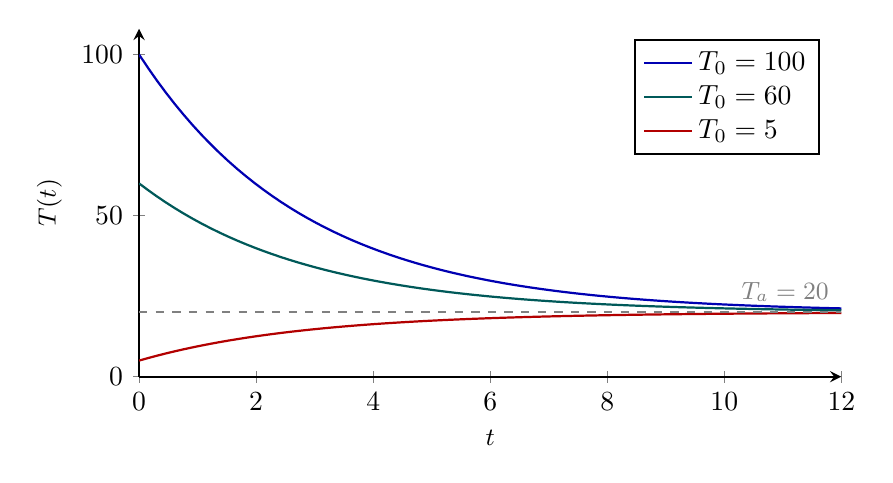
\begin{tikzpicture}
\begin{axis}[
  width=10.5cm, height=6cm,
  xlabel={\small $t$}, ylabel={\small $T(t)$},
  domain=0:12, samples=80,
  ymin=0, ymax=108, xmin=0, xmax=12,
  legend pos=north east, legend cell align=left,
  axis lines=left, thick,
]
\addplot[blue!70!black]{20+80*exp(-0.35*x)}; \addlegendentry{$T_0=100$}
\addplot[teal!70!black]{20+40*exp(-0.35*x)}; \addlegendentry{$T_0=60$}
\addplot[red!70!black]{20-15*exp(-0.35*x)}; \addlegendentry{$T_0=5$}
\addplot[dashed,gray,samples=2]{20} node[pos=0.92,above]{\small $T_a=20$};
\end{axis}
\end{tikzpicture}
\caption{Ley de enfriamiento de Newton \(T(t)=T_a+(T_0-T_a)e^{-kt}\) con \(T_a=20\), \(k=0.35\). Toda curva tiende asintóticamente a la temperatura ambiente; la de \(T_0=5\) corresponde a un cuerpo que se calienta.}
\label{fig:enfriamiento_curvas}
\end{figure}

\begin{example}[Enfriamiento de un objeto]
Un objeto a \(100^\circ\)C se coloca en una habitación a \(20^\circ\)C. Después de 5 minutos su temperatura es \(80^\circ\)C. Encontrar el tiempo necesario para que alcance \(30^\circ\)C.

\begin{myproof}
\textbf{Paso 1.} Modelo: \(\frac{dT}{dt} = -k(T-20)\). Separar:
\[
\frac{dT}{T-20} = -k\,dt.
\]

\textbf{Paso 2.} Integrar:
\[
\ln|T-20| = -kt + C \quad\Rightarrow\quad T(t) = 20 + Ce^{-kt}.
\]
Con \(T(0)=100\): \(100 = 20 + C \Rightarrow C=80\). Luego \(T(t)=20+80e^{-kt}\).

\textbf{Paso 3.} Usar \(T(5)=80\):
\[
80 = 20 + 80e^{-5k} \Rightarrow e^{-5k} = \frac{60}{80} = 0.75 \Rightarrow k = -\frac{\ln 0.75}{5}.
\]

\textbf{Paso 4.} Hallar \(t\) para \(T=30\):
\[
30 = 20 + 80e^{-kt} \Rightarrow e^{-kt} = \frac{10}{80} = 0.125 \Rightarrow t = \frac{\ln 0.125}{-k} = \frac{5\ln 0.125}{\ln 0.75}.
\]
Calculando:
\[
\boxed{t \approx 31.45 \text{ minutos}}.
\]
\end{myproof}
\end{example}

\subsection{Circuito RL con fuente senoidal}
Consideremos ahora \(E(t)=E_0 \sen(\omega t)\). La ecuación es \(L i' + R i = E_0 \sen(\omega t)\). La solución particular se obtiene por coeficientes indeterminados o por factor integrante. El circuito subyacente (Figura~\ref{fig:circuito_rl}) consta de una resistencia \(R\) y una inductancia \(L\) en serie con la fuente; aplicando la ley de voltajes de Kirchhoff, la caída \(Ri\) en la resistencia más la caída \(L\,i'\) en la inductancia igualan al voltaje de la fuente.

\begin{figure}[H]
\centering
\begin{circuitikz}[american, scale=0.95, transform shape]
\draw (0,0) to[sinusoidal voltage source, l=$E(t)$] (0,2.6)
      to[R, l=$R$] (3,2.6)
      to[L, l=$L$, i=$i(t)$] (3,0) -- (0,0);
\end{circuitikz}
\caption{Circuito RL en serie con fuente de voltaje \(E(t)\). La corriente \(i(t)\) satisface \(L\,i'+R\,i=E(t)\).}
\label{fig:circuito_rl}
\end{figure}

\begin{example}[Respuesta forzada senoidal]
Resolver \(i' + \frac{R}{L}i = \frac{E_0}{L}\sen(\omega t)\) con \(i(0)=0\).

\begin{myproof}
\textbf{Paso 1.} Factor integrante \(\mu(t)=e^{(R/L)t}\). Multiplicar:
\[
(e^{(R/L)t} i)' = \frac{E_0}{L} e^{(R/L)t}\sen(\omega t).
\]

\textbf{Paso 2.} Integrar. Usamos la fórmula:
\[
\int e^{at}\sen(\omega t)\,dt = \frac{e^{at}}{a^2+\omega^2}(a\sen\omega t - \omega\cos\omega t).
\]
Aquí \(a=R/L\). Entonces:
\[
e^{(R/L)t} i = \frac{E_0}{L}\cdot \frac{e^{(R/L)t}}{(R/L)^2+\omega^2}\left(\frac{R}{L}\sen\omega t - \omega\cos\omega t\right) + C.
\]

\textbf{Paso 3.} Despejar \(i\):
\[
i(t) = \frac{E_0}{L}\cdot \frac{1}{(R/L)^2+\omega^2}\left(\frac{R}{L}\sen\omega t - \omega\cos\omega t\right) + Ce^{-(R/L)t}.
\]

\textbf{Paso 4.} Aplicar \(i(0)=0\):
\[
0 = \frac{E_0}{L}\cdot \frac{1}{(R/L)^2+\omega^2}\left(-\omega\right) + C \Rightarrow C = \frac{E_0 \omega}{L}\cdot \frac{1}{(R/L)^2+\omega^2}.
\]
Por tanto,
\[
\boxed{i(t) = \frac{E_0}{L}\cdot \frac{1}{(R/L)^2+\omega^2}\left[\frac{R}{L}\sen\omega t - \omega\cos\omega t + \omega e^{-(R/L)t}\right]}.
\]
\end{myproof}
\end{example}

\section{Problemas resueltos adicionales}

% Básico
\begin{prob}
Resolver \(\frac{dy}{dx} = \frac{x}{y}\) con \(y(1)=2\).
\begin{myproof}
\(y\,dy = x\,dx\). Integrar: \(\frac{y^2}{2} = \frac{x^2}{2}+C \Rightarrow y^2 - x^2 = C\). Con \(x=1,y=2\): \(4-1=3\). \(\boxed{y^2 - x^2 = 3}\).
\end{myproof}
\end{prob}

% Básico
\begin{prob}
Resolver \(y' + 3y = 6\).
\begin{myproof}
Factor integrante \(\mu=e^{3x}\). \((e^{3x}y)'=6e^{3x}\). Integrar: \(e^{3x}y=2e^{3x}+C \Rightarrow y=2+Ce^{-3x}\). \(\boxed{y=2+Ce^{-3x}}\).
\end{myproof}
\end{prob}

% Básico
\begin{prob}
Resolver \(y' - y = e^x\).
\begin{myproof}
\(\mu=e^{-x}\). \((e^{-x}y)'=1\). Integrar: \(e^{-x}y=x+C \Rightarrow y=e^x(x+C)\). \(\boxed{y=e^x(x+C)}\).
\end{myproof}
\end{prob}

% Básico
\begin{prob}
Resolver \(y' + \frac{2}{x}y = 3x\).
\begin{myproof}
Lineal: \(\mu=x^2\). \((x^2 y)'=3x^3\). Integrar: \(x^2 y = \frac{3}{4}x^4 + C \Rightarrow y = \frac{3}{4}x^2 + Cx^{-2}\). \(\boxed{y = \frac{3}{4}x^2 + \frac{C}{x^2}}\).
\end{myproof}
\end{prob}

% Básico
\begin{prob}
Resolver \(y' = e^{x-y}\).
\begin{myproof}
Separable: \(e^y dy = e^x dx\). Integrar: \(e^y = e^x + C \Rightarrow y = \ln(e^x+C)\). \(\boxed{y = \ln(e^x+C)}\).
\end{myproof}
\end{prob}

% Básico
\begin{prob}
Resolver \(y' = y^2 \sen x\).
\begin{myproof}
\(\frac{dy}{y^2} = \sen x\,dx\). Integrar: \(-\frac{1}{y} = -\cos x + C \Rightarrow y = \frac{1}{\cos x - C}\). \(\boxed{y = \frac{1}{\cos x - C}}\).
\end{myproof}
\end{prob}

% Básico
\begin{prob}
Resolver \(y' + 2xy = x\).
\begin{myproof}
\(\mu = e^{x^2}\). \((e^{x^2}y)' = x e^{x^2}\). Integrar: \(e^{x^2}y = \frac{1}{2}e^{x^2} + C \Rightarrow y = \frac{1}{2} + Ce^{-x^2}\). \(\boxed{y = \frac{1}{2} + Ce^{-x^2}}\).
\end{myproof}
\end{prob}

% Básico
\begin{prob}
Resolver \(y' = \frac{x^2}{y^2}\).
\begin{myproof}
\(y^2 dy = x^2 dx\). Integrar: \(\frac{y^3}{3} = \frac{x^3}{3} + C \Rightarrow y^3 = x^3 + C\). \(\boxed{y^3 = x^3 + C}\).
\end{myproof}
\end{prob}

% Básico
\begin{prob}
Resolver \(y' = \frac{3x^2 y}{x^3+1}\).
\begin{myproof}
Separable: \(\frac{dy}{y} = \frac{3x^2}{x^3+1}dx\). Integrar: \(\ln|y| = \ln|x^3+1| + C \Rightarrow y = C(x^3+1)\). \(\boxed{y = C(x^3+1)}\).
\end{myproof}
\end{prob}

% Intermedio
\begin{prob}
Resolver \((x^2+y^2)\,dx - 2xy\,dy = 0\).
\begin{myproof}
\(M=x^2+y^2\), \(N=-2xy\). \(M_y=2y\), \(N_x=-2y\) no son iguales, así que no es exacta. Reescribir: \(\frac{dy}{dx} = \frac{x^2+y^2}{2xy} = \frac{x}{2y}+\frac{y}{2x}\), que es homogénea. Sea \(y=vx\): \(v+xv' = \frac{1}{2v}+\frac{v}{2} \Rightarrow xv' = \frac{1-v^2}{2v}\). Separar: \(\frac{2v}{1-v^2}dv = \frac{dx}{x}\). Integrar: \(-\ln|1-v^2| = \ln|x|+C \Rightarrow 1-v^2 = \frac{C}{x}\). Sustituir \(v=y/x\): \(1 - \frac{y^2}{x^2} = \frac{C}{x} \Rightarrow x^2 - y^2 = Cx\). \(\boxed{x^2 - y^2 = Cx}\).
\end{myproof}
\end{prob}

% Intermedio
\begin{prob}
Resolver \(y' = \frac{y}{x} + x^2\).
\begin{myproof}
Lineal: \(y' - \frac{1}{x}y = x^2\). \(\mu = e^{-\ln x}=x^{-1}\). \((x^{-1}y)'=x\). Integrar: \(x^{-1}y = \frac{x^2}{2}+C \Rightarrow y = \frac{x^3}{2}+Cx\). \(\boxed{y = \frac{x^3}{2}+Cx}\).
\end{myproof}
\end{prob}

% Intermedio
\begin{prob}
Resolver \(y' = \frac{2x}{y+x^2 y}\).
\begin{myproof}
Factor \(y+x^2 y = y(1+x^2)\). Entonces \(y' = \frac{2x}{y(1+x^2)}\). Separar: \(y\,dy = \frac{2x}{1+x^2}dx\). Integrar: \(\frac{y^2}{2} = \ln(1+x^2)+C \Rightarrow y^2 = 2\ln(1+x^2)+C\). \(\boxed{y^2 = 2\ln(1+x^2)+C}\).
\end{myproof}
\end{prob}

% Intermedio
\begin{prob}
Resolver \(y' = \frac{2y}{x} + x^2\).
\begin{myproof}
Lineal: \(y' - \frac{2}{x}y = x^2\). \(\mu = x^{-2}\). \((x^{-2}y)' = 1\). Integrar: \(x^{-2}y = x + C \Rightarrow y = x^3 + Cx^2\). \(\boxed{y = x^3 + Cx^2}\).
\end{myproof}
\end{prob}

% Intermedio
\begin{prob}
Resolver \(y' = \frac{y}{x} + \frac{x}{y}\).
\begin{myproof}
Homogénea. \(y=vx\): \(v+xv' = v + \frac{1}{v}\). \(xv' = \frac{1}{v}\). \(v\,dv = \frac{dx}{x}\). Integrar: \(\frac{v^2}{2} = \ln|x| + C \Rightarrow v^2 = 2\ln|x| + C\). Sustituir: \(\frac{y^2}{x^2} = 2\ln|x| + C \Rightarrow y^2 = x^2(2\ln|x| + C)\). \(\boxed{y^2 = x^2(2\ln|x| + C)}\).
\end{myproof}
\end{prob}

% Intermedio
\begin{prob}
Resolver \(y' = \frac{y}{x} - \tan\left(\frac{y}{x}\right)\).
\begin{myproof}
Homogénea: \(y=vx\): \(v+xv' = v - \tan v\). \(xv' = -\tan v\). \(\cot v\, dv = -\frac{dx}{x}\). Integrar: \(\ln|\sen v| = -\ln|x| + C \Rightarrow \sen v = \frac{C}{x}\). Sustituir: \(\boxed{x \sen(y/x) = C}\).
\end{myproof}
\end{prob}

\section{Problemas propuestos}

% Básico
\begin{prob}
Resolver \(y' = 3x^2 y\) con \(y(0)=2\).
\end{prob}

\begin{prob}
Resolver \(\dfrac{dy}{dx} = y\cos x\) con \(y(0)=1\).
\end{prob}

\begin{prob}
Resolver \(y' + y = e^{-x}\).
\end{prob}

\begin{prob}
Un café a \(90^\circ\)C se deja en una sala a \(20^\circ\)C y a los 5 minutos está a \(70^\circ\)C. ¿Qué temperatura tendrá a los 15 minutos?
\end{prob}

% Intermedio
\begin{prob}
Resolver \(y' = \dfrac{1+y^2}{1+x^2}\) con \(y(0)=1\).
\end{prob}

\begin{prob}
Resolver \(xy' - y = x^2\).
\end{prob}

\begin{prob}
Resolver \(y' + \dfrac{1}{x}\,y = \cos x\) para \(x>0\).
\end{prob}

\begin{prob}
Resolver la ecuación exacta \((2xy+1)\,dx + (x^2+3y^2)\,dy = 0\).
\end{prob}

\begin{prob}
Resolver la ecuación exacta \((y\cos x + 2xe^y)\,dx + (\sen x + x^2 e^y - 1)\,dy = 0\).
\end{prob}

\begin{prob}
Resolver la ecuación homogénea \(y' = \dfrac{x^2+y^2}{xy}\).
\end{prob}

\begin{prob}
Un tanque contiene inicialmente 200 L de agua pura. Entra salmuera con \(0.5\) kg/L de sal a razón de 4 L/min y la mezcla bien agitada sale a la misma razón. Determine la cantidad de sal \(x(t)\) en el tanque.
\end{prob}

\begin{prob}
La corriente de un circuito RL satisface \(i' + 2i = 10\) con \(i(0)=0\). Halle \(i(t)\).
\end{prob}

% Desafiante
\begin{prob}
Resolver la ecuación de Bernoulli \(y' + y = x y^2\).
\end{prob}

\begin{prob}
Resolver la ecuación de Bernoulli \(y' + \dfrac{y}{x} = y^3\) para \(x>0\).
\end{prob}

\begin{prob}
Halle las trayectorias ortogonales de la familia de parábolas \(y = Cx^2\).
\end{prob}
